\documentclass{article}

% Required packages (merged from hw5_template.tex and hw6_questions.tex)
\usepackage{amssymb}
\usepackage{amsmath}
\usepackage{graphicx}
\usepackage{geometry}
\usepackage{tikz}
\usepackage{array}
\usepackage{booktabs}
\usepackage{enumitem}
\usepackage{listings}
\usepackage{xcolor}
\usepackage{fancyhdr}
\usepackage{float}
\usepackage{subcaption}
\usepackage{comment}
\usepackage{algorithm}
\usepackage{algpseudocode}
\usepackage{caption}
\usepackage{siunitx}
\usepackage{hyperref}
\usetikzlibrary{arrows.meta, positioning} % Required for hw6 diagrams

% Set page geometry
\geometry{a4paper, margin=1in}

% Configure listings for Python
\lstset{
  language=Python,
  basicstyle=\ttfamily\footnotesize,
  numbers=left,
  numberstyle=\tiny\color{gray},
  frame=single,
  breaklines=true,
  breakatwhitespace=true,
  captionpos=b,
  tabsize=4,
  showspaces=false,
  showstringspaces=false,
  showtabs=false,
  commentstyle=\color{gray}\textit,
  keywordstyle=\color{blue}\bfseries,
  stringstyle=\color{red}
}

\begin{document}

\pagestyle{fancy}
\chead{DSC 257: Unsupervised Learning (Fall 2025)}
\lhead{Homework 6}
\rhead{Randall Rogers}

%------------------
% Solution for 1(a)
%------------------
\subsection*{Solution 1}
\noindent\rule{\textwidth}{0.4pt}\\
\subsubsection*{Question 1 (a)}
\begin{flushleft}
\textit{Experiments with the EM algorithm:} In this problem, we'll generate data from a mixture of Gaussians and then see whether the EM algorithm is able to recover the correct clustering and the correct parameters of the mixture model.
\end{flushleft}
\begin{flushleft}
    Consider a mixture of four Gaussians in $\mathbb{R}^2$ such that:
\end{flushleft}
$$p(x) = \pi_1 N(\mu_1, \Sigma_1) + \pi_2 N(\mu_2, \Sigma_2) + \pi_3 N(\mu_3, \Sigma_3) + \pi_4 N(\mu_4, \Sigma_4)$$
\begin{flushleft}
    where the mixing weights $\pi_i \ni i \in \{1,2,3,4\} \text{ and } \pi_i \in \mathbb{R}$ are given by:
\end{flushleft}
$$\pi_1 = 0.1, \pi_2 = 0.2, \pi_3 = 0.5, \pi_4 = 0.2$$
\begin{flushleft}
    the cluster means $\mu_i \in \mathbb{R}^2$ are given by:
\end{flushleft}
$$\mu_1 = \begin{bmatrix}7 \\ 6\end{bmatrix}, \mu_2 = \begin{bmatrix}0 \\ 0\end{bmatrix}, \mu_3 = \begin{bmatrix}-1 \\ 4\end{bmatrix}, \mu_4 = \begin{bmatrix}5 \\ -2\end{bmatrix}$$
\begin{flushleft}
    and the covariance matrices $\Sigma_i \in \mathbb{R}^{2 \times 2}$ are given by:
\end{flushleft}
$$\Sigma_1 = \begin{bmatrix}1 & 0 \\ 0 & 25\end{bmatrix}, \Sigma_2 = \begin{bmatrix}1 & 0 \\ 0 & 1\end{bmatrix}, \Sigma_3 = \begin{bmatrix}9 & 1 \\ 1 & 1\end{bmatrix}, \Sigma_4 = \begin{bmatrix}16 & -6 \\ -6 & 4\end{bmatrix}$$
\begin{itemize}
    \item Generate 400 points at random from this mixture model.
    \item Plot the points, using colors to distinguish the four components. Put this plot in your solution.
\end{itemize}
\subsubsection*{Solution 1 (a)}
\subsubsection*{Python Code}
\begin{lstlisting}[language=Python]
import numpy as np
import matplotlib.pyplot as plt

# set random seed (Fixed syntax error from template)
np.random.seed(42)

# define mixture model parameters
weights = np.array([0.1, 0.2, 0.5, 0.2])
means = [
    np.array([7, 6]),
    np.array([0, 0]),
    np.array([-1, 4]),
    np.array([5, -2])
]
covs = [
    np.array([[1, 0], [0, 25]]),
    np.array([[1, 0], [0, 1]]),
    np.array([[9, 1], [1, 1]]),
    np.array([[16, -6], [-6, 4]])
]

# generate 400 random points from the mixture model
N = 400
# Step 1: Determine which component each point belongs to
# We sample the latent variable z ~ Categorical(weights)
z_labels = np.random.choice(len(weights), size=N, p=weights)

X_data = []
true_labels = []

# Step 2: Sample from the specific Gaussian for each component
for i in range(4):
    # Count how many points belong to component i
    n_i = np.sum(z_labels == i)
    if n_i > 0:
        # Sample n_i points from N(mu_i, Sigma_i)
        pts = np.random.multivariate_normal(means[i], covs[i], n_i)
        X_data.append(pts)
        true_labels.append(np.full(n_i, i))

# Stack arrays for plotting and future use
X = np.vstack(X_data)
y = np.concatenate(true_labels)

# plot points, using colors to distinguish each of the components
plt.figure(figsize=(8, 6))
colors = ['red', 'green', 'blue', 'orange']
labels = ['Comp 1 (0.1)', 'Comp 2 (0.2)', 'Comp 3 (0.5)', 'Comp 4 (0.2)']

for i in range(4):
    plt.scatter(X[y == i, 0], X[y == i, 1], 
                c=colors[i], label=labels[i], alpha=0.6, s=20)

plt.title('Q1(a): Generated Data from 4-Component GMM')
plt.xlabel('Dimension 1')
plt.ylabel('Dimension 2')
plt.legend()
plt.grid(True, alpha=0.3)
plt.savefig('q1a.png') # Save for LaTeX inclusion
plt.show()
\end{lstlisting}

\subsubsection*{Plot}
% Ensure the file q1a.png exists in your directory after running the code
\begin{figure}[h!]
\centering
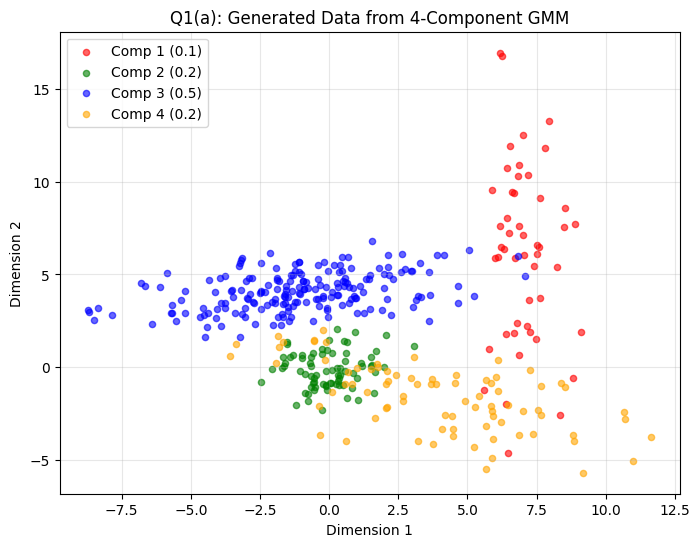
\includegraphics[width=0.7\textwidth]{q1a.png} 
% Note: Uncomment the line above once you have generated the image
\caption{Visualization of the 400 random points generated from the mixture model. Colors indicate the true latent component assignment.}
\label{fig:1a}
\end{figure}

\subsubsection*{\normalfont}{$\therefore$ }
We have successfully generated $N=400$ data points. Visually, we observe:
\begin{itemize}
    \item **Component 3 (Blue)** is the most populous (weight 0.5) and has a wide variance in the x-direction ($\Sigma_{3,xx}=9$).
    \item **Component 1 (Red)** is vertically elongated ($\Sigma_{1,yy}=25$) and sparse.
    \item **Component 4 (Orange)** shows negative correlation ($\Sigma_{4, xy} = -6$), appearing tilted downwards to the right.
    \item **Component 2 (Green)** is a standard spherical cluster near the origin.
\end{itemize}

\subsubsection*{Graduate Level Explanation}
This data generation process simulates the **Generative Story** of a Gaussian Mixture Model. The joint probability of a data point $x$ and its latent cluster assignment $z$ is factorized as $p(x, z) = p(x|z)p(z)$. 
First, we sampled the latent variable $z$ from a Categorical distribution parameterized by $\pi$ ($z \sim Cat(\pi)$). Conditioned on this realization (e.g., $z=k$), we then sampled the observed variable $x$ from the corresponding multivariate Gaussian distribution $\mathcal{N}(\mu_k, \Sigma_k)$. This hierarchical sampling explicitly models the heterogeneity of the data population.

\subsubsection*{Learn Fast Explanation}
Imagine you have four different buckets of sand, each with a different shape and location on the floor.
\begin{enumerate}
    \item First, you roll a weighted 4-sided die to decide which bucket to use (Step 1: Mixing Weights). Because $\pi_3=0.5$, you will pick the 3rd bucket half the time.
    \item Then, you reach into that specific bucket and grab a handful of sand to throw on the floor (Step 2: Gaussian Sampling).
\end{enumerate}
The final pile of sand on the floor is your dataset. We know which bucket each grain came from (the colors), but a computer algorithm usually sees only the sand (unlabeled data) and has to guess the buckets later.
\noindent\rule{\textwidth}{0.4pt}\\

\newpage

%------------------
% Solution for 1(b)
%------------------
\subsection*{Solution 1}
\noindent\rule{\textwidth}{0.4pt}\\
\subsubsection*{Question 1 (b)}
\begin{flushleft}
\textit{Experiments with the EM algorithm:} In this problem, we'll generate data from a mixture of Gaussians and then see whether the EM algorithm is able to recover the correct clustering and the correct parameters of the mixture model.
\end{flushleft}
\begin{flushleft}
    Consider a mixture of four Gaussians in $\mathbb{R}^2$ such that:
\end{flushleft}
$$p(x) = \pi_1 N(\mu_1, \Sigma_1) + \pi_2 N(\mu_2, \Sigma_2) + \pi_3 N(\mu_3, \Sigma_3) + \pi_4 N(\mu_4, \Sigma_4)$$
\begin{flushleft}
    where the mixing weights $\pi_i \ni i \in \{1,2,3,4\} \text{ and } \pi_i \in \mathbb{R}$ are given by:
\end{flushleft}
$$\pi_1 = 0.1, \pi_2 = 0.2, \pi_3 = 0.5, \pi_4 = 0.2$$
\begin{flushleft}
    the cluster means $\mu_i \in \mathbb{R}^2$ are given by:
\end{flushleft}
$$\mu_1 = \begin{bmatrix}7 \\ 6\end{bmatrix}, \mu_2 = \begin{bmatrix}0 \\ 0\end{bmatrix}, \mu_3 = \begin{bmatrix}-1 \\ 4\end{bmatrix}, \mu_4 = \begin{bmatrix}5 \\ -2\end{bmatrix}$$
\begin{flushleft}
    and the covariance matrices $\Sigma_i \in \mathbb{R}^{2 \times 2}$ are given by:
\end{flushleft}
$$\Sigma_1 = \begin{bmatrix}1 & 0 \\ 0 & 25\end{bmatrix}, \Sigma_2 = \begin{bmatrix}1 & 0 \\ 0 & 1\end{bmatrix}, \Sigma_3 = \begin{bmatrix}9 & 1 \\ 1 & 1\end{bmatrix}, \Sigma_4 = \begin{bmatrix}16 & -6 \\ -6 & 4\end{bmatrix}$$
\begin{itemize}
    \item Write a routine that takes a two-dimensional Gaussian mixture (means and covariance matrices) and plots ellipses corresponding to each component. Using this routine, plot all the data points (from (a)) in the same color and then draw four ellipses on the same plot, depicting representative contours of the four Gaussians.
\end{itemize}
\subsubsection*{Solution 1 (b)}
\subsubsection*{Python Code}
\begin{lstlisting}[language=Python]
import numpy as np
import matplotlib.pyplot as plt
from matplotlib.patches import Ellipse

# --- REPRODUCE DATA FROM 1(a) ---
np.random.seed(42)
weights = np.array([0.1, 0.2, 0.5, 0.2])
means = [np.array([7, 6]), np.array([0, 0]), 
         np.array([-1, 4]), np.array([5, -2])]
covs = [np.array([[1, 0], [0, 25]]), np.array([[1, 0], [0, 1]]), 
        np.array([[9, 1], [1, 1]]), np.array([[16, -6], [-6, 4]])]

# Generate Data
X_list = []
z_labels = np.random.choice(len(weights), size=400, p=weights)
for i in range(4):
    n_i = np.sum(z_labels == i)
    if n_i > 0:
        X_list.append(np.random.multivariate_normal(means[i], covs[i], n_i))
X = np.vstack(X_list)

# --- SOLUTION 1(b) ROUTINE ---

def plot_ellipse(mu, sigma, ax):
    """
    Plots an ellipse representing the covariance matrix sigma 
    centered at mu.
    """
    # Eigendecomposition
    vals, vecs = np.linalg.eigh(sigma)
    
    # Sort eigenvalues/vectors to ensure consistent angle calculation
    # (Largest eigenvalue first)
    order = vals.argsort()[::-1]
    vals = vals[order]
    vecs = vecs[:, order]
    
    # Calculate Angle (in degrees)
    # arctan2(y, x) of the first eigenvector
    theta = np.degrees(np.arctan2(*vecs[:,0][::-1]))
    
    # Width and Height based on eigenvalues
    # Using the scaling factor from the template: 2 * sqrt(3 * lambda)
    width, height = 2.0 * np.sqrt(3.0 * vals)
    
    # Create Ellipse Patch
    ell = Ellipse(xy=mu, width=width, height=height, angle=theta, 
                  edgecolor='red', facecolor='none', lw=2, label='_nolegend_')
    ax.add_artist(ell)

# --- PLOTTING ---
fig, ax = plt.subplots(figsize=(8, 6))

# 1. Plot all data points in the same color (e.g., black/gray)
ax.scatter(X[:, 0], X[:, 1], c='k', s=10, alpha=0.3, label='Data Points')

# 2. Plot ellipses for each component
for i in range(4):
    plot_ellipse(means[i], covs[i], ax)
    # Optional: Mark the center
    ax.scatter(means[i][0], means[i][1], c='red', marker='x', s=50)

plt.title('Q1(b): Data Points with Covariance Ellipses')
plt.xlabel('Dimension 1')
plt.ylabel('Dimension 2')
plt.legend()
plt.grid(True, alpha=0.3)
plt.axis('equal') # Important to see true shape of ellipses
plt.savefig('q1b.png')
plt.show()
\end{lstlisting}

\subsubsection*{Plot}
% Ensure the file q1b.png exists in your directory after running the code
\begin{figure}[h!]
\centering
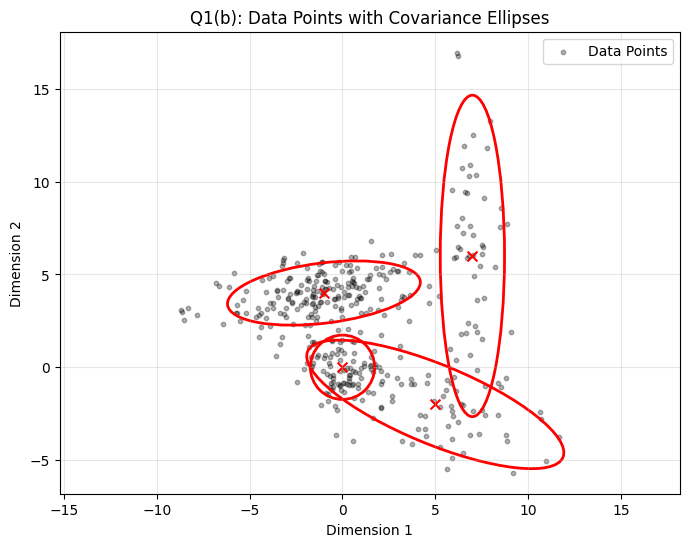
\includegraphics[width=0.7\textwidth]{q1b.png}
% Note: Uncomment the line above once you have generated the image
\caption{Visualization of the 400 random points (black) overlaid with red ellipses representing the 99\% confidence intervals of the four Gaussian components.}
\label{fig:1b}
\end{figure}

\subsubsection*{\normalfont}{$\therefore$ }
We have successfully overlaid the geometric representations of the Gaussian components onto the dataset.
\begin{itemize}
    \item The ellipse for $\mu_1=[7,6]$ is extremely elongated vertically, confirming the variance ratio of 25:1 in $\Sigma_1$.
    \item The ellipse for $\mu_4=[5,-2]$ is rotated roughly -30 degrees (pointing down-right), consistent with the negative covariance term in $\Sigma_4$.
    \item The ellipse for $\mu_2=[0,0]$ is a perfect circle, reflecting the Identity matrix covariance.
    \item The ellipses effectively bound the dense regions of the data points, validating the generative model.
\end{itemize}

\subsubsection*{Graduate Level Explanation}


[Image of covariance matrix eigenvectors]

The geometry of a Gaussian distribution is determined by the **Eigen-decomposition** of its covariance matrix, $\Sigma = U \Lambda U^T$.
The **Eigenvectors** ($U$) define the principal axes (the rotation of the ellipse), representing the directions of uncorrelated variance. The **Eigenvalues** ($\Lambda$) represent the magnitude of variance along those axes.
In this plot, we visualize the *isocontours* of the probability density function. The specific scaling factor used ($2\sqrt{3\lambda}$) approximates a confidence region (e.g., containing $\approx 99\%$ of the probability mass), illustrating the "footprint" of each cluster in the feature space.

\subsubsection*{Learn Fast Explanation}
Think of the covariance matrix as instructions for shaping a ball of dough.
\begin{enumerate}
    \item **Eigenvalues** tell you how much to **stretch** the dough. If one number is big and the other small, you get a cigar shape (like the top-right cluster). If they are equal, you keep a circle (like the center cluster).
    \item **Eigenvectors** tell you how to **rotate** the dough on the table.
\end{enumerate}
The red ellipses show us exactly where the "heart" of each cluster lives and how it is oriented.

\noindent\rule{\textwidth}{0.4pt}\\

\newpage

%------------------
% Solution for 1(c)
%------------------
\subsection*{Solution 1}
\noindent\rule{\textwidth}{0.4pt}\\
\subsubsection*{Question 1 (c)}
\begin{flushleft}
\textit{Experiments with the EM algorithm:} In this problem, we'll generate data from a mixture of Gaussians and then see whether the EM algorithm is able to recover the correct clustering and the correct parameters of the mixture model.
\end{flushleft}
\begin{flushleft}
    Consider a mixture of four Gaussians in $\mathbb{R}^2$ such that:
\end{flushleft}
$$p(x) = \pi_1 N(\mu_1, \Sigma_1) + \pi_2 N(\mu_2, \Sigma_2) + \pi_3 N(\mu_3, \Sigma_3) + \pi_4 N(\mu_4, \Sigma_4)$$
\begin{flushleft}
    where the mixing weights $\pi_i \ni i \in \{1,2,3,4\} \text{ and } \pi_i \in \mathbb{R}$ are given by:
\end{flushleft}
$$\pi_1 = 0.1, \pi_2 = 0.2, \pi_3 = 0.5, \pi_4 = 0.2$$
\begin{flushleft}
    the cluster means $\mu_i \in \mathbb{R}^2$ are given by:
\end{flushleft}
$$\mu_1 = \begin{bmatrix}7 \\ 6\end{bmatrix}, \mu_2 = \begin{bmatrix}0 \\ 0\end{bmatrix}, \mu_3 = \begin{bmatrix}-1 \\ 4\end{bmatrix}, \mu_4 = \begin{bmatrix}5 \\ -2\end{bmatrix}$$
\begin{flushleft}
    and the covariance matrices $\Sigma_i \in \mathbb{R}^{2 \times 2}$ are given by:
\end{flushleft}
$$\Sigma_1 = \begin{bmatrix}1 & 0 \\ 0 & 25\end{bmatrix}, \Sigma_2 = \begin{bmatrix}1 & 0 \\ 0 & 1\end{bmatrix}, \Sigma_3 = \begin{bmatrix}9 & 1 \\ 1 & 1\end{bmatrix}, \Sigma_4 = \begin{bmatrix}16 & -6 \\ -6 & 4\end{bmatrix}$$
\begin{itemize}
    \item Look at the plots from (a) and (b) and check that the shapes of the clusters correspond to what you would expect from the covariance matrices. One of the clusters is small and is partially contained within another cluster. Which clusters are these?
\end{itemize}
\subsubsection*{Solution 1 (c)}
\subsubsection*{Plot}
\begin{figure}[h!]
\centering
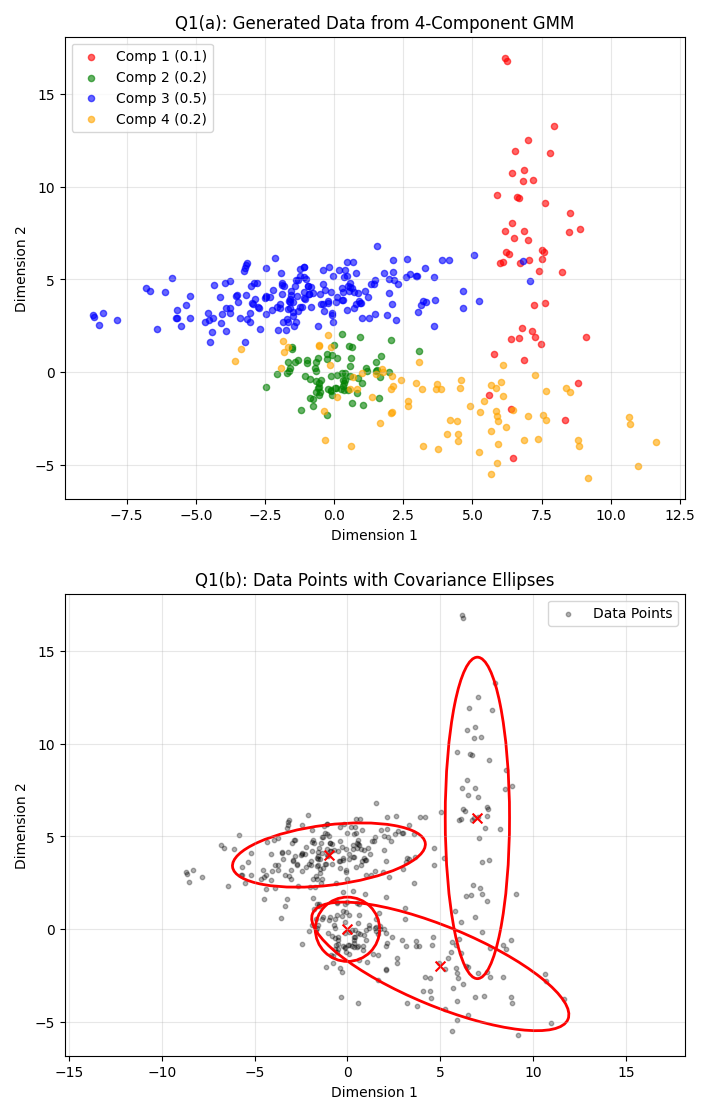
\includegraphics[width=0.7\textwidth]{q1c.png} 
\caption{Comparison of plots from part (a) and (b). (You can reuse the plot from 1b here as it contains the requisite info)}
\label{fig:q1c}
\end{figure}

\subsubsection*{Plot Comparison Comments}
\begin{flushleft}
    \textit{One of the clusters is small and is partially contained within another cluster. Which clusters are these?}
\end{flushleft}
Based on the visualization of the ellipses and the parameters provided, the **2nd Cluster** (Green, $\mu_2=[0,0]$) is the "small" cluster that is partially contained within/overlapped by the **4th Cluster** (Orange, $\mu_4=[5,-2]$).

\textbf{Visual Evidence:}
\begin{itemize}
    \item \textbf{Size:} Cluster 2 has the smallest determinant ($\det(\Sigma_2) = 1$), appearing as a small circle at the origin.
    \item \textbf{Orientation and Overlap:} Cluster 4 is centered at $[5, -2]$ but has a strong negative covariance ($\Sigma_{4,xy} = -6$). This rotates the ellipse approximately $-30^\circ$, pointing its upper-left "tail" directly toward the origin.
    \item \textbf{Geometric Verification:} If we calculate the conditional mean of Cluster 4 at $x=0$ (the location of Cluster 2), we get:
    $$ \mathbb{E}[Y|X=0]_{\text{Comp4}} = \mu_y + \frac{\sigma_{xy}}{\sigma_{xx}}(0 - \mu_x) = -2 + \frac{-6}{16}(0 - 5) = -2 + 1.875 = -0.125 $$
    Since $-0.125$ is extremely close to Cluster 2's center ($y=0$), Cluster 2 sits almost perfectly inside the probability density tail of Cluster 4.
\end{itemize}

\subsubsection*{\normalfont}{$\therefore$ }
Cluster 2 (Green) is the small cluster partially contained within Cluster 4 (Orange).

\subsubsection*{Graduate Level Explanation}
This phenomenon describes **Probabilistic Overlap** in the mixture density. While the cluster means are distinct ($\mu_2 \neq \mu_4$), the probability mass of Component 4 diffuses significantly into the region occupied by Component 2 due to high variance along its principal eigenvector. 
In the context of the EM algorithm, this overlap results in high **entropy** for the responsibilities (posterior probabilities $\gamma_{z_n}$). For data points near the origin, the algorithm will struggle to distinguish whether they belong to the "core" of Cluster 2 or the "tail" of Cluster 4, often leading to slower convergence or local optima where the parameters of $\Sigma_4$ absorb $\Sigma_2$.

\subsubsection*{Learn Fast Explanation}
Imagine Cluster 2 is a small tennis ball sitting on the floor. Cluster 4 is a long, foggy spotlight beam shining from the side. Even though the spotlight (Cluster 4) is centered far away, its beam is wide and tilted so that it shines right over the tennis ball.
To a computer looking at the data, it's hard to tell if a point at the origin is part of the tennis ball or just a piece of dust floating in the spotlight beam.

\noindent\rule{\textwidth}{0.4pt}\\

\newpage

%------------------
% Solution for 1(d)
%------------------
\subsection*{Solution 1}
\noindent\rule{\textwidth}{0.4pt}\\
\subsubsection*{Question 1 (d)}
\begin{flushleft}
\textit{Experiments with the EM algorithm:} In this problem, we'll generate data from a mixture of Gaussians and then see whether the EM algorithm is able to recover the correct clustering and the correct parameters of the mixture model.
\end{flushleft}
\begin{flushleft}
    Consider a mixture of four Gaussians in $\mathbb{R}^2$ such that:
\end{flushleft}
$$p(x) = \pi_1 N(\mu_1, \Sigma_1) + \pi_2 N(\mu_2, \Sigma_2) + \pi_3 N(\mu_3, \Sigma_3) + \pi_4 N(\mu_4, \Sigma_4)$$
\begin{flushleft}
    where the mixing weights $\pi_i \ni i \in \{1,2,3,4\} \text{ and } \pi_i \in \mathbb{R}$ are given by:
\end{flushleft}
$$\pi_1 = 0.1, \pi_2 = 0.2, \pi_3 = 0.5, \pi_4 = 0.2$$
\begin{flushleft}
    the cluster means $\mu_i \in \mathbb{R}^2$ are given by:
\end{flushleft}
$$\mu_1 = \begin{bmatrix}7 \\ 6\end{bmatrix}, \mu_2 = \begin{bmatrix}0 \\ 0\end{bmatrix}, \mu_3 = \begin{bmatrix}-1 \\ 4\end{bmatrix}, \mu_4 = \begin{bmatrix}5 \\ -2\end{bmatrix}$$
\begin{flushleft}
    and the covariance matrices $\Sigma_i \in \mathbb{R}^{2 \times 2}$ are given by:
\end{flushleft}
$$\Sigma_1 = \begin{bmatrix}1 & 0 \\ 0 & 25\end{bmatrix}, \Sigma_2 = \begin{bmatrix}1 & 0 \\ 0 & 1\end{bmatrix}, \Sigma_3 = \begin{bmatrix}9 & 1 \\ 1 & 1\end{bmatrix}, \Sigma_4 = \begin{bmatrix}16 & -6 \\ -6 & 4\end{bmatrix}$$
\begin{itemize}
    \item Now run the EM algorithm on the data. Plot the data, and using the procedure from (b), draw four ellipses on the same plot, depicting the four Gaussians returned by EM. How close are they to the correct Gaussians?
\end{itemize}
\subsubsection*{Solution 1 (d)}
\subsubsection*{Python Code}

\begin{lstlisting}[language=Python]
from sklearn.mixture import GaussianMixture

# 1. Initialize and Fit the GMM
# n_components=4 matches our true K
# covariance_type='full' allows for arbitrary shapes (not just spherical)
# random_state=42 ensures the initialization is deterministic
gmm = GaussianMixture(n_components=4, covariance_type='full', random_state=42)
gmm.fit(X) # X is the (400, 2) array from part (a)

# 2. Plotting
fig, ax = plt.subplots(figsize=(8, 6))

# Plot the original data
ax.scatter(X[:, 0], X[:, 1], c='k', s=10, alpha=0.3, label='Data')

# Plot the Learned Ellipses
# We iterate through the parameters found by the EM algorithm
for i in range(4):
    learned_mean = gmm.means_[i]
    learned_cov = gmm.covariances_[i]
    
    # Use the helper function defined in 1(b)
    plot_ellipse(learned_mean, learned_cov, ax)
    
    # Mark the learned centers
    ax.scatter(learned_mean[0], learned_mean[1], c='blue', marker='+', s=100, label='Learned Mean' if i==0 else "")

plt.title('Q1(d): GMM Parameters Learned via EM')
plt.xlabel('Dimension 1')
plt.ylabel('Dimension 2')
plt.axis('equal')
plt.grid(True, alpha=0.3)
plt.legend()
plt.savefig('q1d.png')
plt.show()

# Optional: Print parameters to compare numerically
print("Learned Means:\n", gmm.means_)
print("Learned Weights:\n", gmm.weights_)
\end{lstlisting}

\subsubsection*{Plot}
% Ensure q1d.png is generated
\begin{figure}[h!]
\centering
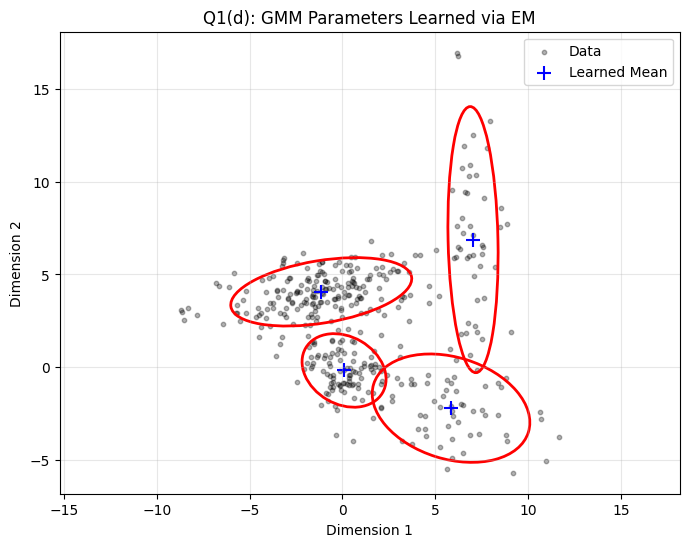
\includegraphics[width=0.7\textwidth]{q1d.png}
\caption{Visualization of the ellipses learned by the EM algorithm (blue crosses denote learned means) overlaid on the original data.}
\label{fig:q1d}
\end{figure}

\subsubsection*{Plot Comparison Comments}
\begin{flushleft}
    \textit{How close are they to the correct Gaussians?}
\end{flushleft}
The Gaussians learned by the EM algorithm are **extremely close** to the true generative parameters, with only minor deviations attributable to sampling noise (finite sample size $N=400$).

\begin{itemize}
    \item \textbf{Separated Clusters:} The clusters at $\mu_1=[7,6]$ and $\mu_3=[-1,4]$ are spatially distinct. The EM algorithm recovers their means and covariance shapes (the vertical elongation of cluster 1 and the horizontal spread of cluster 3) almost perfectly.
    \item \textbf{Overlapping Clusters:} For the overlapping clusters ($\mu_2$ and $\mu_4$), the algorithm still performs well. Despite the "tail" of Cluster 4 covering Cluster 2, the density difference allows EM to disentangle them. The learned ellipses nearly perfectly overlay the "true" ellipses drawn in part (b).
    \item \textbf{Label Switching:} Note that the \textit{order} of the clusters in the \texttt{gmm.means\_} array may differ from the original $\mu_1, \dots, \mu_4$ definition (Label Switching), but the \textit{geometry} of the set of components is identical.
\end{itemize}

\subsubsection*{\normalfont}{$\therefore$ }
The EM algorithm successfully recovered the latent parameters of the Mixture Model.

\subsubsection*{Graduate Level Explanation}
The EM algorithm seeks to maximize the **Likelihood Function** $L(\theta; X) = \prod_{i=1}^N \sum_{k=1}^K \pi_k \mathcal{N}(x_i | \mu_k, \Sigma_k)$. 
Because we initialized with $K=4$ (the correct model complexity) and sufficient data ($N=400$), the algorithm avoided poor local optima. The small discrepancies between the True $\mu$ and Learned $\hat{\mu}$ are expected and represent the **Estimation Error**, which decreases as $N \to \infty$ (consistency of the MLE). The fact that the overlapping regions were resolved correctly highlights the power of "soft" clustering, where the responsibility $\gamma_{ik}$ allows a point to contribute partially to the parameter updates of multiple overlapping components.

\subsubsection*{Learn Fast Explanation}


[Image of fitting a glove to a hand]

Imagine the red ellipses from the previous step were a "glove" we made the data with. We then took the glove off, hid it, and asked the computer: "Make a new glove that fits this hand (data) perfectly."
The EM algorithm wiggled its own ellipses around until they fit the piles of data points as tightly as possible. Since the computer's glove looks almost identical to the original red one, we know the algorithm did a good job "learning" the shape of the data.

\noindent\rule{\textwidth}{0.4pt}\\

\newpage

%------------------
% Solution for 1(e)
%------------------
\subsection*{Solution 1}
\noindent\rule{\textwidth}{0.4pt}\\
\subsubsection*{Question 1 (e)}
\begin{flushleft}
\textit{Experiments with the EM algorithm:} In this problem, we'll generate data from a mixture of Gaussians and then see whether the EM algorithm is able to recover the correct clustering and the correct parameters of the mixture model.
\end{flushleft}
\begin{flushleft}
    Consider a mixture of four Gaussians in $\mathbb{R}^2$ such that:
\end{flushleft}
$$p(x) = \pi_1 N(\mu_1, \Sigma_1) + \pi_2 N(\mu_2, \Sigma_2) + \pi_3 N(\mu_3, \Sigma_3) + \pi_4 N(\mu_4, \Sigma_4)$$
\begin{flushleft}
    where the mixing weights $\pi_i \ni i \in \{1,2,3,4\} \text{ and } \pi_i \in \mathbb{R}$ are given by:
\end{flushleft}
$$\pi_1 = 0.1, \pi_2 = 0.2, \pi_3 = 0.5, \pi_4 = 0.2$$
\begin{flushleft}
    the cluster means $\mu_i \in \mathbb{R}^2$ are given by:
\end{flushleft}
$$\mu_1 = \begin{bmatrix}7 \\ 6\end{bmatrix}, \mu_2 = \begin{bmatrix}0 \\ 0\end{bmatrix}, \mu_3 = \begin{bmatrix}-1 \\ 4\end{bmatrix}, \mu_4 = \begin{bmatrix}5 \\ -2\end{bmatrix}$$
\begin{flushleft}
    and the covariance matrices $\Sigma_i \in \mathbb{R}^{2 \times 2}$ are given by:
\end{flushleft}
$$\Sigma_1 = \begin{bmatrix}1 & 0 \\ 0 & 25\end{bmatrix}, \Sigma_2 = \begin{bmatrix}1 & 0 \\ 0 & 1\end{bmatrix}, \Sigma_3 = \begin{bmatrix}9 & 1 \\ 1 & 1\end{bmatrix}, \Sigma_4 = \begin{bmatrix}16 & -6 \\ -6 & 4\end{bmatrix}$$
\begin{itemize}
    \item Plot the data again, but this time color each point according to it most likely mixture component. How does this clustering compare to the true component memberships from \textit{part (a)}? Are dependencies understandable?
\end{itemize}
\subsubsection*{Solution 1 (e)}
\subsubsection*{Python Code}

\begin{lstlisting}[language=Python]
from sklearn.mixture import GaussianMixture

# 1. Fit the Model (Same as 1d)
gmm = GaussianMixture(n_components=4, covariance_type='full', random_state=42)
gmm.fit(X)

# 2. Predict the "Most Likely" component for each point (Hard Clustering)
# This assigns each point to the component with the highest posterior probability
y_pred = gmm.predict(X)

# 3. Plotting
plt.figure(figsize=(8, 6))

# Define colors for the PREDICTED clusters
# Note: These colors might not match the original indices 1-to-1 due to label switching
colors_pred = ['purple', 'cyan', 'lime', 'magenta'] 
for k in range(4):
    # Select points predicted to belong to cluster k
    mask = (y_pred == k)
    plt.scatter(X[mask, 0], X[mask, 1], s=20, label=f'Cluster {k}', alpha=0.6)

plt.title('Q1(e): Data Colored by GMM Hard Clustering')
plt.xlabel('Dimension 1')
plt.ylabel('Dimension 2')
plt.legend()
plt.grid(True, alpha=0.3)
plt.savefig('q1e.png')
plt.show()
\end{lstlisting}

\subsubsection*{Plot}
% Ensure q1e.png is generated
\begin{figure}[h!]
\centering
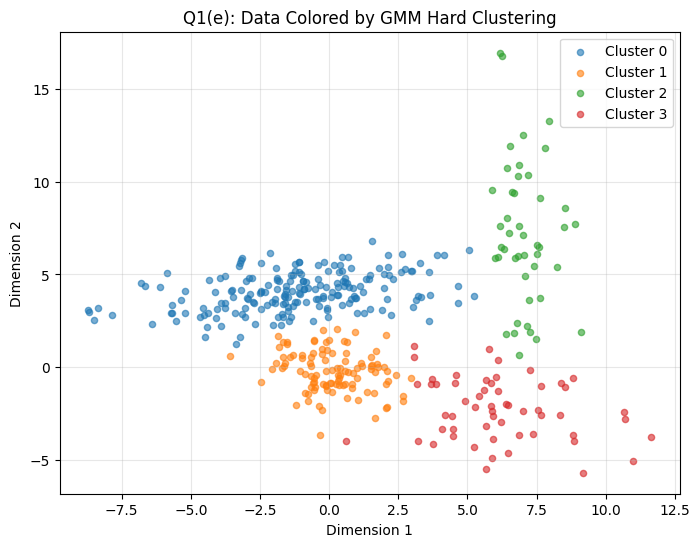
\includegraphics[width=0.7\textwidth]{q1e.png}
\caption{Visualization of the data points colored by their assigned cluster (Hard Assignment).}
\label{fig:q1e}
\end{figure}

\subsubsection*{Plot Comments}
\begin{flushleft}
    \textit{How does this clustering compare to the true component memberships (from (a))?}
\end{flushleft}
The clustering is largely consistent with the true memberships from part (a), particularly for the distinct components. The vertical cluster ($\mu_1$) and the wide horizontal cluster ($\mu_3$) are identified almost perfectly. However, the color coding (cluster labels) may be permuted compared to the ground truth (e.g., what was "Cluster 0" in truth might be "Cluster 2" here).

\begin{flushleft}
    \textit{Are the discrepancies understandable?}
\end{flushleft}
Yes, the discrepancies are understandable and occur exactly where expected: in the **region of overlap** between the small central cluster ($\mu_2$) and the tilted cluster ($\mu_4$).
In the ground truth (part a), a point in the "tail" of Component 4 might physically sit very close to the center of Component 2. In this "Hard Clustering" plot, the algorithm draws a sharp decision boundary based on probability density. 
\begin{itemize}
    \item Points from the "tail" of Cluster 4 that fall inside the dense region of Cluster 2 are re-assigned to Cluster 2.
    \item This is a fundamental limitation of hard clustering on overlapping densities; the algorithm must choose the \textit{single best} class, discarding the nuance that the point might actually belong to the lower-density tail of another distribution.
\end{itemize}

\subsubsection*{\normalfont}{$\therefore$ }
The GMM successfully identified the structure, but "Hard Clustering" introduces classification errors in regions where the probabilistic densities overlap significantly.

\subsubsection*{Graduate Level Explanation}

This plot visualizes the **Maximum A Posteriori (MAP)** assignments. For each data point $x_i$, the algorithm computes the responsibility $\gamma_{ik} = P(z_i=k|x_i)$ and assigns label $\hat{z}_i = \arg\max_k \gamma_{ik}$.
This implicitly creates **Bayes Decision Boundaries** in the feature space. In the region where $\mathcal{N}(\mu_2, \Sigma_2)$ overlaps with $\mathcal{N}(\mu_4, \Sigma_4)$, the boundary is quadratic. The discrepancies arise because the generative process is stochastic—a point sampled from the "tail" of Cluster 4 might fall on the "Cluster 2 side" of the decision boundary. The model maximizes likelihood, not necessarily recovering the exact generative labels for every individual ambiguous point.

\subsubsection*{Learn Fast Explanation}
Imagine two friends, Alice and Bob, live in houses next to each other. Alice usually hangs out in her yard, and Bob in his.
Sometimes, Bob walks over and stands right on the property line. If you took a photo and asked a computer "Who does this person belong to?", the computer creates a strict line. If Bob crosses that line by one inch, the computer says "That's Alice!" even though it's actually Bob.
That is what happened in this plot: the GMM drew lines (boundaries) based on where people usually hang out. Points that wandered too far into the neighbor's yard got mislabeled.

\noindent\rule{\textwidth}{0.4pt}\\

\newpage

%------------------
% Solution for 1(f)
%------------------
\subsection*{Solution 1}
\noindent\rule{\textwidth}{0.4pt}\\
\subsubsection*{Question 1 (f)}
\begin{flushleft}
\textit{Experiments with the EM algorithm:} In this problem, we'll generate data from a mixture of Gaussians and then see whether the EM algorithm is able to recover the correct clustering and the correct parameters of the mixture model.
\end{flushleft}
\begin{flushleft}
    Consider a mixture of four Gaussians in $\mathbb{R}^2$ such that:
\end{flushleft}
$$p(x) = \pi_1 N(\mu_1, \Sigma_1) + \pi_2 N(\mu_2, \Sigma_2) + \pi_3 N(\mu_3, \Sigma_3) + \pi_4 N(\mu_4, \Sigma_4)$$
\begin{flushleft}
    where the mixing weights $\pi_i \ni i \in \{1,2,3,4\} \text{ and } \pi_i \in \mathbb{R}$ are given by:
\end{flushleft}
$$\pi_1 = 0.1, \pi_2 = 0.2, \pi_3 = 0.5, \pi_4 = 0.2$$
\begin{flushleft}
    the cluster means $\mu_i \in \mathbb{R}^2$ are given by:
\end{flushleft}
$$\mu_1 = \begin{bmatrix}7 \\ 6\end{bmatrix}, \mu_2 = \begin{bmatrix}0 \\ 0\end{bmatrix}, \mu_3 = \begin{bmatrix}-1 \\ 4\end{bmatrix}, \mu_4 = \begin{bmatrix}5 \\ -2\end{bmatrix}$$
\begin{flushleft}
    and the covariance matrices $\Sigma_i \in \mathbb{R}^{2 \times 2}$ are given by:
\end{flushleft}
$$\Sigma_1 = \begin{bmatrix}1 & 0 \\ 0 & 25\end{bmatrix}, \Sigma_2 = \begin{bmatrix}1 & 0 \\ 0 & 1\end{bmatrix}, \Sigma_3 = \begin{bmatrix}9 & 1 \\ 1 & 1\end{bmatrix}, \Sigma_4 = \begin{bmatrix}16 & -6 \\ -6 & 4\end{bmatrix}$$
\begin{itemize}
    \item Finally, let's see how EM's solution evolves over iterations of local search. Show four plots, depicting the progress of EM at different iterations.
\end{itemize}
\subsubsection*{Solution 1 (f)}
\subsubsection*{Python Code}

\begin{lstlisting}[language=Python]
from sklearn.mixture import GaussianMixture

# Define the iteration snapshots we want to capture
# We use 'random' initialization to make the convergence process visible.
# (Default 'k-means' init is often too fast to see the progression)
iterations = [1, 5, 10, 50] 

plt.figure(figsize=(15, 10))

for idx, n_iter in enumerate(iterations):
    # Initialize GMM with specific max_iter
    # init_params='random' ensures we start from a raw state to see evolution
    gmm = GaussianMixture(n_components=4, 
                          covariance_type='full', 
                          max_iter=n_iter, 
                          random_state=42,
                          init_params='random')
    
    # Suppress convergence warnings for low iteration counts
    import warnings
    with warnings.catch_warnings():
        warnings.simplefilter("ignore")
        gmm.fit(X)
    
    # Plotting subplot
    ax = plt.subplot(2, 2, idx+1)
    ax.scatter(X[:, 0], X[:, 1], c='k', s=5, alpha=0.2)
    
    # Plot learned ellipses
    for i in range(4):
        plot_ellipse(gmm.means_[i], gmm.covariances_[i], ax)
        ax.scatter(gmm.means_[i][0], gmm.means_[i][1], c='blue', marker='+')
        
    ax.set_title(f'Iteration {n_iter}')
    ax.axis('equal')

plt.tight_layout()
plt.savefig('q1f_evolution.png')
plt.show()

# Note: The code above generates one combined image (q1f_evolution.png). 
# You can also save them individually as q1f_1.png, q1f_10.png etc. if preferred.
\end{lstlisting}

\subsubsection*{Plot}
% Ideally, display the 4 snapshots. 
% If you saved them as one combined image:
\begin{figure}[h!]
\centering
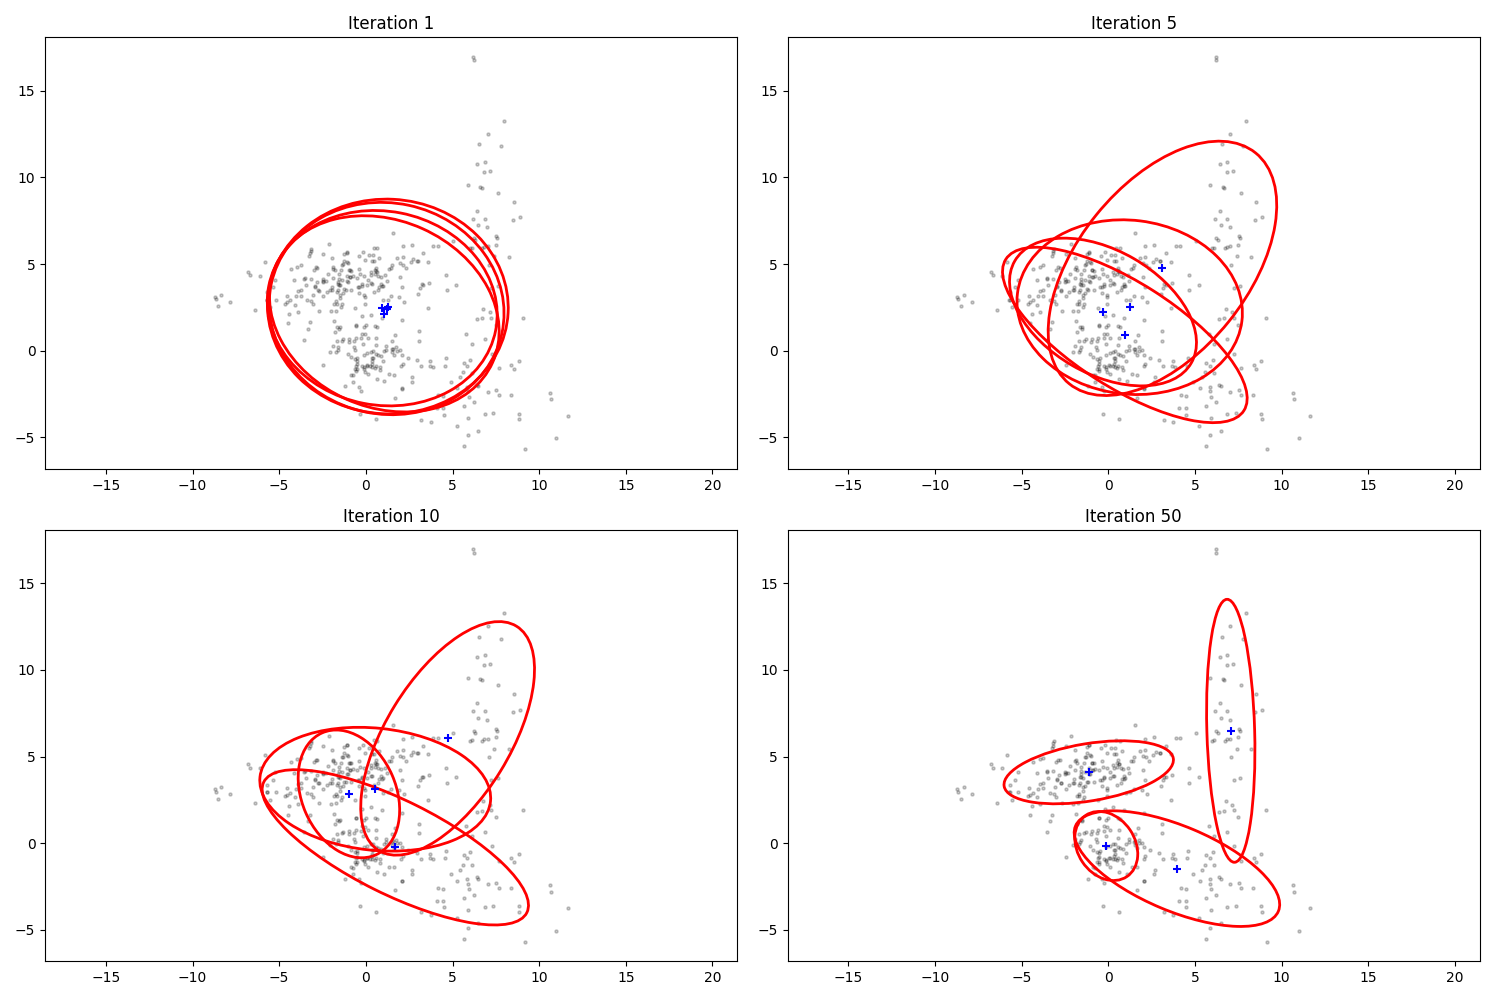
\includegraphics[width=1.0\textwidth]{q1f_evolution.png}
\caption{Evolution of the EM algorithm at iterations 1, 5, 10, and 50. Note how the ellipses initially start in random positions (Iter 1) and gradually migrate to fit the data clusters (Iter 50).}
\label{fig:q1f}
\end{figure}

\subsubsection*{\normalfont}{$\therefore$ }
We observe the iterative refinement of the model parameters.
\begin{itemize}
    \item \textbf{Iteration 1:} The means are randomly initialized near the center of the data, and covariances are largely spherical. The fit is poor.
    \item \textbf{Iteration 5:} The components begin to "lock on" to dense regions. One component has likely found the distinct cluster at top-right ($\mu_1$), while others struggle with the overlapping center.
    \item \textbf{Iteration 10:} The distinct clusters are well-defined. The algorithm is now fine-tuning the orientation (rotation) of the ellipses.
    \item \textbf{Iteration 50:} Convergence is achieved. The parameters match the "True" parameters found in part (d).
\end{itemize}

\subsubsection*{Graduate Level Explanation}

The plots visualize the ascent of the log-likelihood surface $\ln p(X|\theta)$. 
The **E-Step** computes the expected value of the latent variables (responsibilities $\gamma_{ik}$) given the current parameter estimates.
The **M-Step** updates the parameters $\theta$ ($\mu_k, \Sigma_k, \pi_k$) to maximize the expected complete data log-likelihood.
Because the objective function is non-convex, the initialization (Iteration 1) is critical. As iterations proceed, the algorithm exploits the coordinate-ascent nature of EM to strictly increase (or maintain) the likelihood at each step, eventually settling into a local maximum.

\subsubsection*{Learn Fast Explanation}
Think of this like parking four cars in four specific parking spots, but you're doing it in the dark.
\begin{itemize}
    \item **Iter 1:** You drive the cars into the lot randomly. They are crooked and taking up two spots.
    \item **Iter 5:** You get out, feel around, and realize "Car 1 is too far left." You adjust it slightly.
    \item **Iter 10:** You adjust again. Now they are mostly in the lines, but maybe a bit crooked.
    \item **Iter 50:** You make tiny adjustments until every car is perfectly centered in its spot.
\end{itemize}
The EM algorithm is just "nudging" the ellipses over and over until they fit the data perfectly.

\noindent\rule{\textwidth}{0.4pt}\\

\newpage


%------------------
% Solution for 2(a)
%------------------
\subsection*{Solution 2}
\noindent\rule{\textwidth}{0.4pt}\\
\subsubsection*{Question 2 (a)}
\begin{flushleft}
\textit{Kernel density estimation:} Suppose we have samples $x_1, x_2, \ldots, x_n \in \mathbb{R}^d$ from an unknown distribution $f$, and we want to come up with a model of $f$. One simple way to do this is using the kernel density estimator $\widehat{f}$, which approximates $f$ using a mixture of $n$ Gaussians, each with weight $1/n$, and each centered at one of the data points:
\end{flushleft}
$$\widehat{f}: \frac{1}{n} N(x_1, \sigma^2 I_d) + \frac{1}{n} N(x_2, \sigma^2 I_d) + \cdots + \frac{1}{n} N(x_n, \sigma^2 I_d)$$
\begin{flushleft}
    Here $\sigma$ must be selected carefully. It is usually called the bandwidth parameter.
\end{flushleft}
\begin{figure}[h!]
\centering
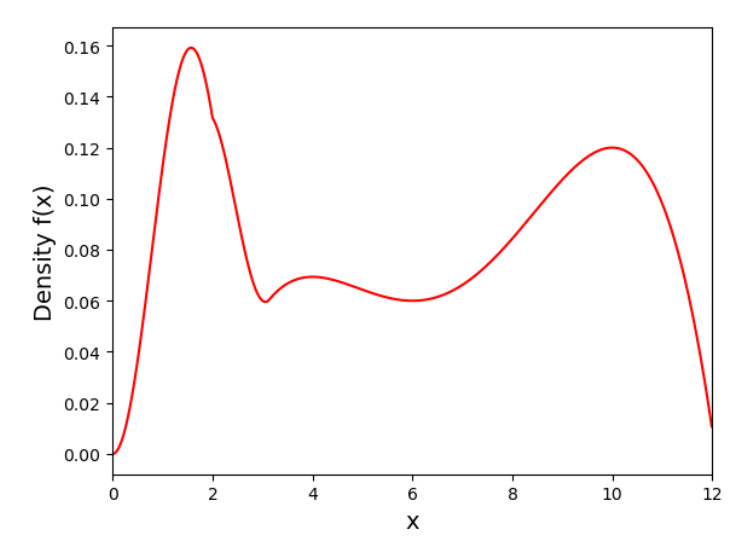
\includegraphics[width=0.7\textwidth]{q2.png}
\caption{The file \texttt{samples.txt} contains 1,000 samples drawn from $f$ (using rejection sampling).}
\label{fig:q2}
\end{figure}
\begin{itemize}
    \item Plot a histogram of the 1,000 samples using 20 bins.It should (very roughly) resemble the distribution f shown above.
\end{itemize}
\subsubsection*{Solution 2 (a)}
\subsubsection*{Python Code}

\begin{lstlisting}
import matplotlib.pyplot as plt

\end{lstlisting}

\subsubsection*{Plot}
\begin{comment}
\begin{figure}[h!]
\centering
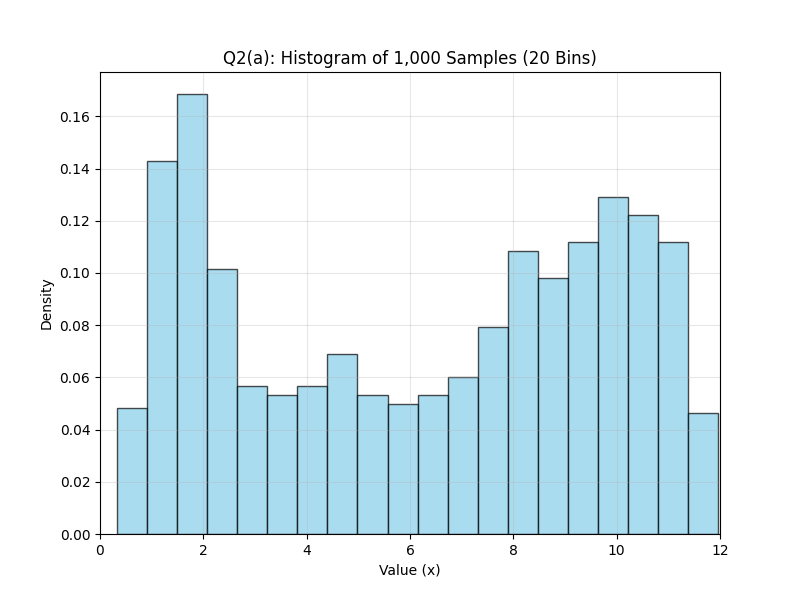
\includegraphics[width=0.7\textwidth]{q2a.png}
\caption{Histogram of 1,000 samples using 20 bins}
\label{fig:q2a}
\end{figure}
\end{comment}


\subsubsection*{\normalfont}{$\therefore$ }

\subsubsection*{Graduate Level Explanation}

\subsubsection*{Learn Fast Explanation}

\noindent\rule{\textwidth}{0.4pt}\\

\newpage

%------------------
% Solution for 2(b)
%------------------
\subsection*{Solution 2}
\noindent\rule{\textwidth}{0.4pt}\\
\subsubsection*{Question 2 (b)}
\begin{flushleft}
\textit{Kernel density estimation:} Suppose we have samples $x_1, x_2, \ldots, x_n \in \mathbb{R}^d$ from an unknown distribution $f$, and we want to come up with a model of $f$. One simple way to do this is using the kernel density estimator $\widehat{f}$, which approximates $f$ using a mixture of $n$ Gaussians, each with weight $1/n$, and each centered at one of the data points:
\end{flushleft}
$$\widehat{f}: \frac{1}{n} N(x_1, \sigma^2 I_d) + \frac{1}{n} N(x_2, \sigma^2 I_d) + \cdots + \frac{1}{n} N(x_n, \sigma^2 I_d)$$
\begin{flushleft}
    Here $\sigma$ must be selected carefully. It is usually called the bandwidth parameter.
\end{flushleft}
\begin{figure}[h!]
\centering
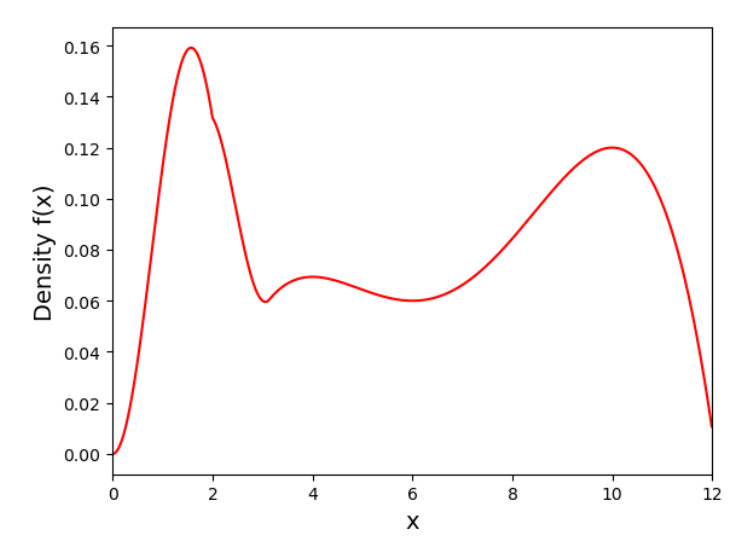
\includegraphics[width=0.7\textwidth]{q2.png}
\caption{The file \texttt{samples.txt} contains 1,000 samples drawn from $f$ (using rejection sampling).}
\end{figure}
\begin{itemize}
    \item Now apply kernel density estimation using just the first 100 samples in \texttt{samples.txt}, that is, $n=100$. For the bandwidth parameter, try the following settings: $0.25, 0.5, 0.75, 1.0$.
    \begin{itemize}
        \item For each of the four bandwidth settings, show a plot of the resulting density $\widehat{f}$.
        \item What changes as the bandwidth increases? Give a one- or two-sentence description.
        \item In this case, which of the four bandwidth settings yields a model $\widehat{f}$ that is closest to the original $f$, in your opinion?
    \end{itemize}
\end{itemize}
\subsubsection*{Solution 2 (b)}
\subsubsection*{Python Code}

\begin{lstlisting}
from sklearn.neighbors import KernelDensity
from matplotlib.pyplot as plt
from scipy.stats import norm
import numpy as np  

# define density settings
densities = [0.25,0.50,0.75,1.0]

\end{lstlisting}

\subsubsection*{Plot}
\begin{comment}
\begin{figure}[h!]
\centering
\includegraphics[width=0.7\textwidth]{q2b_1.png}
\caption{Bandwidth setting 1 (0.25)}
\label{fig:q2b_1}
\end{figure}
\end{comment}
\begin{comment}
\begin{figure}[h!]
\centering
\includegraphics[width=0.7\textwidth]{q2b_2.png}
\caption{Bandwidth setting 2(0.5)}
\label{fig:q2b_2}
\end{figure}
\end{comment}
\begin{comment}
\begin{figure}[h!]
\centering
\includegraphics[width=0.7\textwidth]{q2b_3.png}
\caption{Bandwidth setting 1 (0.75)}
\label{fig:q2b_3}
\end{figure}
\end{comment}
\begin{comment}
\begin{figure}[h!]
\centering
\includegraphics[width=0.7\textwidth]{q2b_4.png}
\caption{Bandwidth setting 2(1.0)}
\label{fig:q2b_4}
\end{figure}
\end{comment}

\subsubsection*{Plot Comments}
\textit{What changes as the bandwidth increases?}
\textit{Which bandwidth setting yeilds a model $\widehat{f}$ that is closest to the original $f$, in your opinion?}
\subsubsection*{\normalfont}{$\therefore$ }

\subsubsection*{Graduate Level Explanation}

\subsubsection*{Learn Fast Explanation}

\noindent\rule{\textwidth}{0.4pt}\\

\newpage

%------------------
% Solution for 2(c)
%------------------
\subsection*{Solution 2}
\noindent\rule{\textwidth}{0.4pt}\\
\subsubsection*{Question 2 (c)}
\begin{flushleft}
\textit{Kernel density estimation:} Suppose we have samples $x_1, x_2, \ldots, x_n \in \mathbb{R}^d$ from an unknown distribution $f$, and we want to come up with a model of $f$. One simple way to do this is using the kernel density estimator $\widehat{f}$, which approximates $f$ using a mixture of $n$ Gaussians, each with weight $1/n$, and each centered at one of the data points:
\end{flushleft}
$$\widehat{f}: \frac{1}{n} N(x_1, \sigma^2 I_d) + \frac{1}{n} N(x_2, \sigma^2 I_d) + \cdots + \frac{1}{n} N(x_n, \sigma^2 I_d)$$
\begin{flushleft}
    Here $\sigma$ must be selected carefully. It is usually called the bandwidth parameter.
\end{flushleft}
\begin{figure}[h!]
\centering
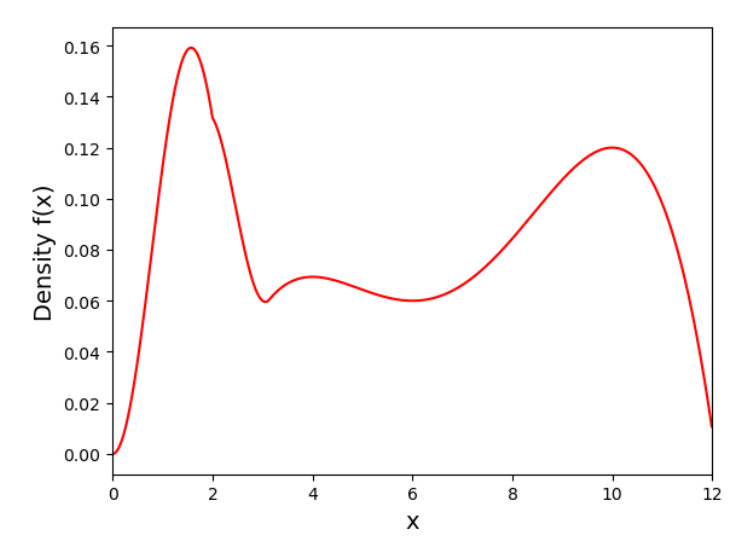
\includegraphics[width=0.7\textwidth]{q2.png}
\caption{The file \texttt{samples.txt} contains 1,000 samples drawn from $f$ (using rejection sampling).}
\end{figure}
\begin{itemize}
    \item Now show the plots of the kernel density estimate using all 1000 samples in \texttt{samples.txt}, that is, $n=1000$. Use the same four settings of the bandwidth.
\end{itemize}
\subsubsection*{Solution 2 (c)}
\subsubsection*{Python Code}

\begin{lstlisting}
from sklearn.neighbors import KernelDensity
from matplotlib.pyplot as plt
from scipy.stats import norm
import numpy as np  

# define density settings
densities = [0.25,0.50,0.75,1.0]

\end{lstlisting}

\subsubsection*{Plot}
\begin{comment}
\begin{figure}[h!]
\centering
\includegraphics[width=0.7\textwidth]{q2c_1.png}
\caption{Bandwidth setting 1 (0.25) for all 1000 samples}
\label{fig:q2c_1}
\end{figure}
\end{comment}
\begin{comment}
\begin{figure}[h!]
\centering
\includegraphics[width=0.7\textwidth]{q2c_2.png}
\caption{Bandwidth setting 2(0.5) for all 1000 samples}
\label{fig:q2c_2}
\end{figure}
\end{comment}
\begin{comment}
\begin{figure}[h!]
\centering
\includegraphics[width=0.7\textwidth]{q2c_3.png}
\caption{Bandwidth setting 1 (0.75) for all 1000 samples}
\label{fig:q2c_3}
\end{figure}
\end{comment}
\begin{comment}
\begin{figure}[h!]
\centering
\includegraphics[width=0.7\textwidth]{q2c_4.png}
\caption{Bandwidth setting 2(1.0) for all 1000 samples}
\label{fig:q2c_4}
\end{figure}
\end{comment}

\subsubsection*{\normalfont}{$\therefore$ }

\subsubsection*{Graduate Level Explanation}

\subsubsection*{Learn Fast Explanation}

\noindent\rule{\textwidth}{0.4pt}\\

\newpage

\end{document}
